\documentclass[11pt]{article}
\usepackage[paperwidth=8.5in, paperheight=11in]{geometry}

\usepackage{../tjimo}

\begin{comment}
\def\answer{\comment}
\def\solution{\comment}
\def\solutionone{\comment}
\def\solutiontwo{\comment}
\end{comment}

\newcommand{\sevenpoints}{Time limit: 30 minutes.}
\newcommand{\righthead}{\fdbox{Round}{Team}}

\begin{document}

\begin{problem}
% (1.5) (2016azhang) 
Upon reaching level 19, Kangaskhan can learn the move ``Double Hit'', which hits twice and deals $x$ damage per hit. However, upon Mega-Evolving into Kangaskhan-Mega, Kangaskhan gains a special ability that allows it to use each move twice, with the second instance of the move dealing half damage. If Kangaskhan-Mega deals 105 damage in total using Double Hit, find $x$.
\end{problem}

\begin{answer}
\boxed{35}.
\end{answer}

\begin{solution}
If Kangaskhan-Mega uses Double Hit without its special ability, it will deal $2x$ damage. With its special ability, it will deal $x$ additional damage. Thus, $2x + x = 105$, and we get $x = \boxed{35}$ (which is actually true.)
\end{solution}

\begin{problem}
% (2.5) (2016skim) 
In triangle ABC, AB = 12 feet and BC = 10 feet. If the altitude of ABC from side AB is equal to 5 feet, what is the altitude of ABC from side BC in feet?
\end{problem}

\begin{answer}
\boxed{6} feet.
\end{answer}

\begin{solution}
The area of a triangle is $\frac{1}{2}bh$, where $b$ is a base of a triangle and $h$ is the base's corresponding height. Looking at the base of 5, the area is $\frac{1}{2} \times 12 \times 5 = 30$. Looking at the other pair, the area is $\frac{1}{2} \times 10h$. Thus, $\frac{1}{2} \times 10 h = 30$, so $h = \boxed{6}$ feet.
\end{solution}

\begin{problem}
% (2.5) (2016azhang) 
Cubone is chopping up a cube with side length 3 in. into 27 little cubes with side length 1 in. Find the minimum number of straight cuts this takes, if Cubone can rearrange pieces that have been chopped off in any manner.
\end{problem}

\begin{answer}
\boxed{6}.
\end{answer}

\begin{solution}
Cubone can chop the cube with side length 3 in. into 27 unit cubes with 6 straight cuts; imagine cutting up a Rubik's Cube. Thus we know our answer must be less than or equal to 6. However, note that the unit cube in the center of the 3 in. cube can only be obtained by at least 6 cuts, no matter how we rearrange the leftover pieces. Thus, the minimum number of cuts is 6 cuts.
\end{solution}

\begin{problem}
% (2.5) (2016skim + 2016azhang) 
Alan, Allen, Allan, Chang, Cheng, and Ch@ng are standing in line to buy tickets for a movie. However, Allen and Cheng insist on standing next to each other. How many ways can the 6 people stand in line?
\end{problem}

\begin{answer}
\boxed{240}.
\end{answer}

\begin{solution}
We can think of Allen and Cheng as one person, since they need to be next to each other. This gives us $5! = 120$ ways of arranging them. We also need to multiply by 2 at the end to account for the arrangement of Allen and Cheng: either AllenCheng or ChengAllen. This gives us $120\cdot2 = \boxed{240}$.
\end{solution}

\begin{problem}
% (3) (2016azhang) 
Ships Jendy and Sam6 are racing down a 500 km waterway. Jendy is going full speed ahead at 30 km/hr, but the captain of Sam6, Mr. Skim, is currently sleeping and has set the ship Sam6 on autopilot at 20 km/hr. When Mr. Skim wakes up, he instantly increases Sam6's speed to 45 km/hr in an effort to catch up. What is the maximum time in hours Mr. Skim can spend sleeping to be able to catch up to Jendy by the end of the race?
\end{problem}

\begin{answer}
\boxed{\frac{107}{13}}.
\end{answer}

\begin{solution}
We have that Jendy finishes in $\frac{500 \text{ km}}{30 \text{ km/hr}} = \frac{50}{3}$ hours, so Sam6 must also finish in $\frac{50}{3}$ hours in order to catch up to Jendy. Let $x$ denote the maximum time in hours that Mr. Skim can spend sleeping. Then, $\frac{50}{3} - x$ denotes the time in hours that Mr. Skim is awake and sailing Sam6 at 45 km/hr. Thus, we have that $20x + 45(\frac{50}{3}-x) = 500$. Solving gives us $x = \boxed{\frac{107}{13}}$.
\end{solution}

\begin{problem}
% (3.5) (2016azhang) 
Pikachu is facing off against Blissey, who has a high special defense. Luckily, Pikachu knows the move Charge Beam, which has a 70 percent chance of boosting Pikachu's special attack by 1 stage. What is the probability that Pikachu gets at least 2 special attack boosts in 3 moves?
\end{problem}

\begin{answer}
\boxed{\frac{98}{125}}.
\end{answer}

\begin{solution}
Let Y denote the event that Pikachu gets a special attack boost from one use of Charge Beam, and let N denote the event that Pikachu doesn't get a special attack boost from one Charge Beam. Then, to have at least 2 special attack boosts in 3 moves, we need one of the following sequences: YYN, YNY, NYY, or YYY. YYN, YNY, and NYY each have a $(\frac{7}{10})^2\cdot\frac{3}{10}$ probability of happening, while YYY has a $(\frac{7}{10})^3$ probability of happening. Summing the probabilities of all 4 sequences gives us $3\cdot(\frac{7}{10})^2\cdot\frac{3}{10} + (\frac{7}{10})^3 = \boxed{\frac{98}{125}}$.
\end{solution}

\begin{problem}
% (4) (2016azhang) 
Find the number of factors of 60300 that are divisible by 30.
\end{problem}

\begin{answer}
\boxed{16}.
\end{answer}

\begin{solution}
60300 has a prime factorization of $2^2\cdot3^2\cdot5^2\cdot67$. A factor of 60300 can only be the product of one number in every set of the following: $\{2^0, 2^1, 2^2\}, \{3^0, 3^1, 3^2\}, \{5^0, 5^1, 5^2\}$, and $\{67^0, 67^1\}$. For a factor to be divisible by $30 = 2\cdot3\cdot5$, we must choose $2^1$ or $2^2$ from the first set, $3^1$ or $3^2$ from the second set, and $5^1$ or $5^2$ from the third set; we can choose any number from the last set. Thus, our answer is $2\cdot2\cdot2\cdot2 = 16$.
\end{solution}

\begin{problem}
% (4) (2016azhang) 
Kevlin and Kelvin are playing a game where they normally each start out with 1500 points. However, both of them think 1500 is a boring number, so they decide to each start out with a random real number of points from 0 to 2000, determined by a computer randomizer. However, if the difference in points between them is over 1800, they will run the computer randomizer again. What is the probability that they won't have to run the computer randomizer again? 
\end{problem}

\begin{answer}
\boxed{\frac{99}{100}}.
\end{answer}

\begin{solution}
We can picture the probability space of Kevlin's and Kelvin's money on a coordinate grid. Take the first quadrant of the Cartesian plane; let the $x$-value denote Kevlin's points and let the $y$-value denote Kelvin's points. The probability space is thus the square with coordinates (0, 0), (2000, 0), (0, 2000), and (2000, 2000). We can then see that the regions where the point difference is over 1800 is the shaded area in the diagram below:

\begin{center}
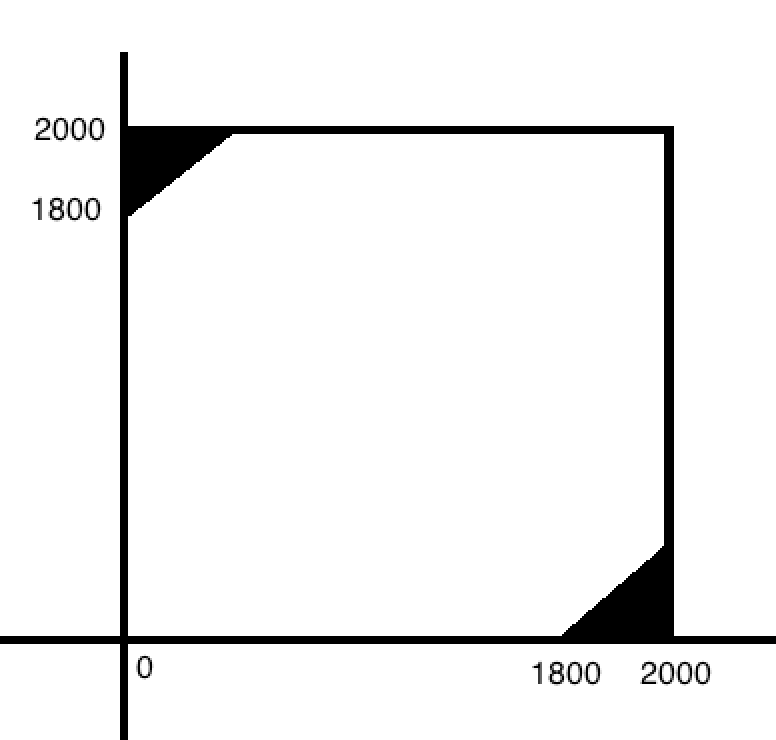
\includegraphics[width=9cm]{probspace.png}
\end{center}

The shaded area thus has a total area of two triangles of base 200 and height 200, or a total of $2\cdot\frac{1}{2}\cdot200\cdot200 = 40000$. The total area of the probability space is $2000\cdot2000=400000$. Thus, the probability that we need to run the computer randomizer again is $\frac{40000}{400000} = \frac{1}{100}$. However, we want the probability that we don't need to run the computer randomizer again, which is $1 - \frac{1}{100} = \boxed{\frac{99}{100}}$.
\end{solution}

\begin{problem}
% (5) (2016azhang) 
Let $x^2 = 7 + 4\sqrt{3}$ and $y^2 = 7 - 4\sqrt{3}$. There are then four distinct values of $x-y$. What is the minimum value of these four values?
\end{problem}

\begin{answer}
\boxed{-4}.
\end{answer}

\begin{solution}
Note that $7 + 4\sqrt{3} = (2 + \sqrt{3})^2$ and $7 - 4\sqrt{3} = (2 - \sqrt{3})^2$. Then, we have $x = \pm(2 + \sqrt{3})$ and $y = \pm(2 - \sqrt{3})$. The four values of $x-y$ are then $2\sqrt{3}$, $4$, $-4$, and $-2\sqrt{3}$, and the minimum of these values is \boxed{-4}.
\end{solution}

\begin{problem}
% (5) (2016skim + 2016azhang) 
A shuriken-shaped design is made by cutting off four quarter-circles from the corners of a square of side length 8 inches. A circle is then inscribed in the shuriken, as shown below. Find the area of the shuriken outside the circle, in square inches.
\begin{center}
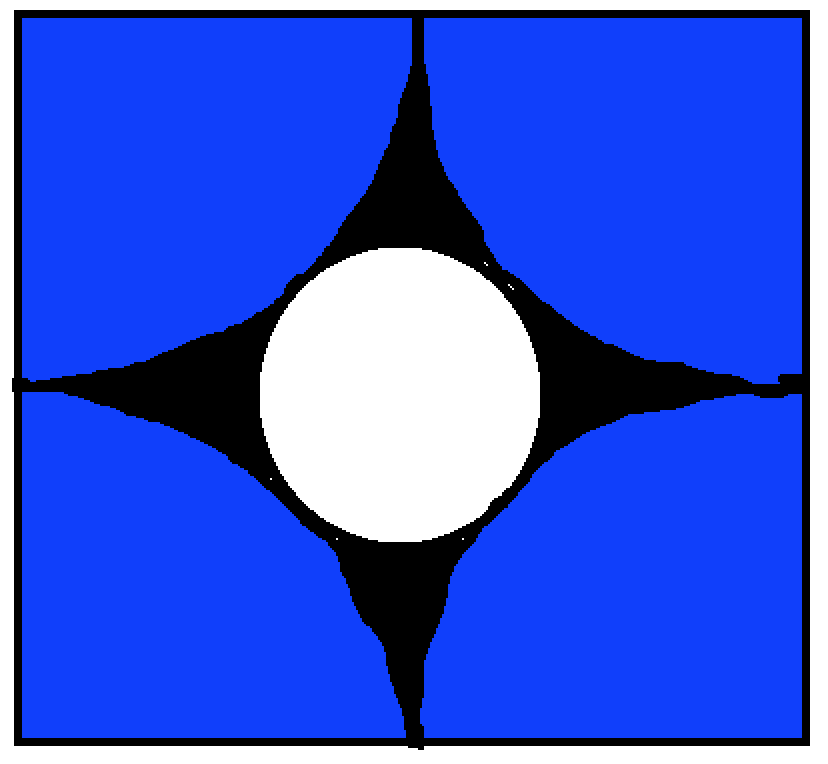
\includegraphics[width=9cm]{shuriken.png}
\end{center}
\end{problem}

\begin{answer}
\boxed{64 - 64\pi + 32\sqrt{2}\pi}.
\end{answer}

\begin{solution}
The non-shuriken area is made up of 4 quarter-circles, which is equal to 1 circle of the same radius in area. Let the radius of this circle be $r$. Then $r^{2}\pi = 16\pi$, so $r = 4$. The shuriken area is thus the area of a square with side length $2r = 8$ minus the shaded area, or $64 - 16\pi$.

To solve for the area outside the circle in the shuriken, we need to find the area of the circle. Let the radius of the inner circle be $R$. Consider a diagonal of the square, with length $8\sqrt{2}$. It is made up of $r$, $2R$, and then $r$ again. Thus, $2r + 2R = 8\sqrt{2}$. Solving for $R$ gives $R = 4\sqrt{2} - 4$, and thus the area of the inner circle is $R^2\pi = 48\pi - 32\sqrt{2}\pi$. Subtracting this from the shuriken's area, $64 - 16\pi$, gives us the final answer of \boxed{64 - 64\pi + 32\sqrt{2}\pi}.
\end{solution}
\end{document}
